%%%%%%%%%%%%%%%%%%%%%%%%%%%%%%%%%%%%%%%%%%%%%%%%%%%%%%%%%%%%%%%%%%%%%
% LaTeX Template: Project Titlepage Modified (v 0.1) by rcx
%
% Original Source: http://www.howtotex.com
% Date: February 2014
% 
% This is a title page template which be used for articles & reports.
% 
% This is the modified version of the original Latex template from
% aforementioned website.
% 
%%%%%%%%%%%%%%%%%%%%%%%%%%%%%%%%%%%%%%%%%%%%%%%%%%%%%%%%%%%%%%%%%%%%%%

\documentclass[12pt]{report}
\usepackage[a4paper]{geometry}
\usepackage[myheadings]{fullpage}
\usepackage{fancyhdr}
\usepackage{lastpage}
\usepackage{graphicx, wrapfig, subcaption, setspace, booktabs}
\usepackage[T1]{fontenc}
\usepackage[font=small, labelfont=bf]{caption}
\usepackage{fourier}
\usepackage[protrusion=true, expansion=true]{microtype}
\usepackage[english]{babel}
\usepackage{sectsty}
\usepackage{url, lipsum}
\usepackage{color,soul} % Highlighting
\usepackage{mathtools} % Math!
\usepackage{environ} % For Large equation block
\usepackage[numbers]{natbib}

\NewEnviron{large_eq}{%
    \begin{equation}
    \scalebox{1.3}{$\BODY$}
    \end{equation}
    }

\newcommand{\HRule}[1]{\rule{\linewidth}{#1}}
\onehalfspacing
\setcounter{tocdepth}{5}
\setcounter{secnumdepth}{5}

%-------------------------------------------------------------------------------
% HEADER & FOOTER
%-------------------------------------------------------------------------------
\pagestyle{fancy}
\fancyhf{}
\setlength\headheight{15pt}
%\fancyhead[L]{Student ID: 1034511}
\fancyhead[R]{The Puzzler}
\fancyfoot[R]{Page \thepage\ of \pageref{LastPage}}
%-------------------------------------------------------------------------------

% TITLE PAGE
%-------------------------------------------------------------------------------

\begin{document}

\title{ \normalsize \textsc{Project Proposal}
		\\ [2.0cm]
		\HRule{0.5pt} \\
		\LARGE \textbf{\uppercase{The Puzzler}}
		\HRule{2pt} \\ [0.5cm]
		\normalsize \today \vspace*{5\baselineskip}}

\date{}

\author{
		CprE 575 - Computational Perception \\
		Alex Luehm \& David Wehr }

\maketitle
\tableofcontents
\newpage

%-------------------------------------------------------------------------------
% Section title formatting
\sectionfont{\scshape}
%-------------------------------------------------------------------------------

%-------------------------------------------------------------------------------
% BODY
%-------------------------------------------------------------------------------

\section*{Introduction}
\addcontentsline{toc}{section}{Introduction}
Jigsaw puzzles have been a favorite table-top pastime for generations - allowing friends and family to constructively work together and enjoy one another's company. In addition, puzzles have become a popular way for individuals to unwind after a stressful day at the office. 

Individuals typically start out with simple, smaller puzzles - usually of around 100 - 300 pieces - and gradually progress to larger puzzle ranges. As the size of puzzles increase, so does the complexity in shape and color of the pieces. It soon becomes more of a burden than an activity to enjoy, causing frustration when progress seems to have come to a standstill.

The puzzle that once brought relaxation and enjoyment now becomes a sore in the room - taking up space and constantly demanding attention. The feeling of guilt begins to feel overpowering when walking into the room and upon seeing the pieces still needing to be sorted and slotted into their respective places. The puzzle needs to be completed, but the friction has become too great.

The Puzzler is designed to alleviate this sense of dread and frustration. Designed for both avid and novice puzzlers alike, The Puzzler will aid its users in finding potential candidate pieces given a selected region of a partially completed puzzle. Through edge detection and piece profiling of detected curves and angles, The Puzzler will suggest potential next-pieces from the pool of yet-unused pieces.


\subsection*{Example Use Case}
\addcontentsline{toc}{subsection}{Use Case}
Ideally, the user will interact with The Puzzler through an Android application. The user will indicate to the app which region it should find pieces for by first taking a picture of the desired region followed by highlighting the specific edge via the device's touch-screen, as seen in Figure \ref{fig:target_piece}. The app will then allow the user to take a picture of the remaining puzzle pieces. 

After characterizing the curve of the desired region and processing the remaining pieces, the app will determine which pieces are most likely to fit the specified region and will indicate them to the user with a visual overlay, for example, highlighting them in red, as shown in Figure \ref{fig:highlighted_piece}.

Beyond finding matching pieces to a partially assembled puzzle, because of our curve description, the application would also be able to find potential matches to single pieces, even if they are not part of an assembled puzzle. Profiles for each captured piece will be recreated on every use - eliminating the need to track pieces and allowing new data for the user for every iteration.

\begin{figure}
\centering
\begin{minipage}{.47\textwidth}
  \centering
  \includegraphics[width=.9\linewidth]{figures/target_piece_cropped.jpg}
  \captionof{figure}{The desired location is highlighted by the user in the application}
  \label{fig:target_piece}
\end{minipage}%
\hfill{}%
\begin{minipage}{.47\textwidth}
  \centering
  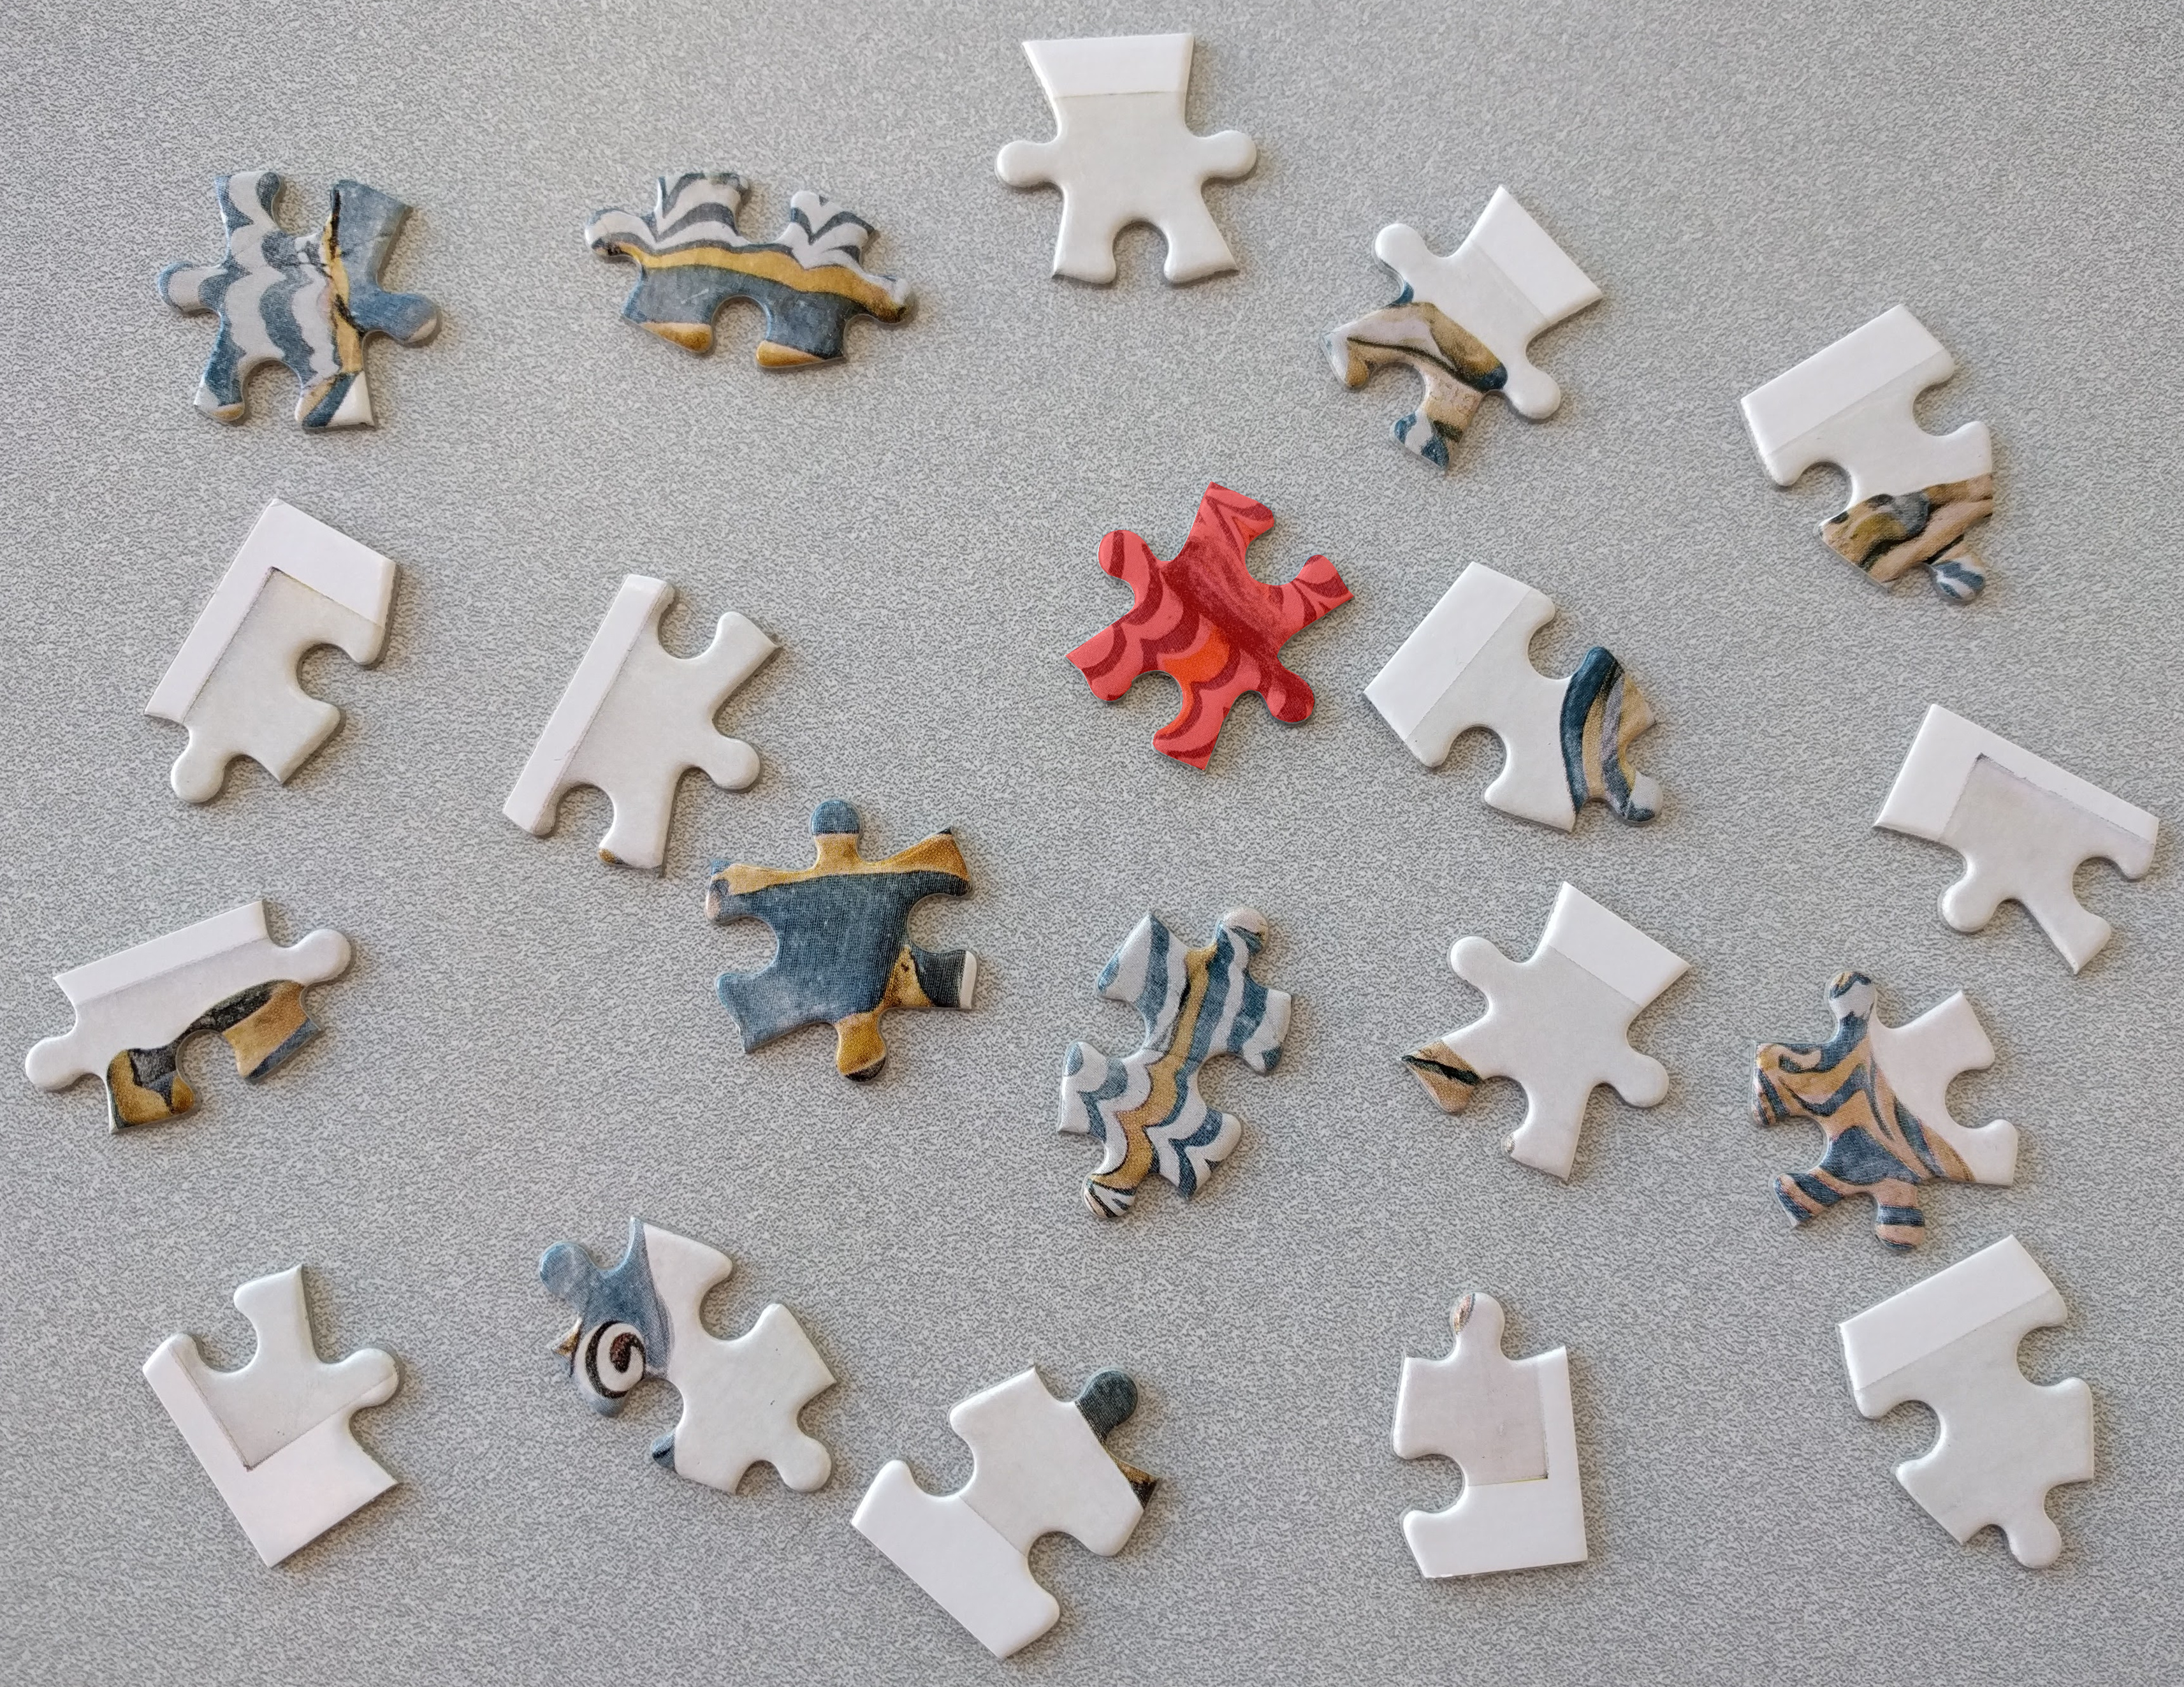
\includegraphics[width=.85\linewidth]{figures/highlighted_piece.jpg}
  \captionof{figure}{The application identifies one or more potential fitting pieces}
  \label{fig:highlighted_piece}
\end{minipage}
\end{figure}

\subsection*{Potential Applications}
\addcontentsline{toc}{subsection}{Applications}
Outside of puzzle solving, there are other applications for algorithms related to jigsaw puzzle solving. In addition to solving entire puzzles, the identification of pieces and their correct global position can be extended to reconstructing artifacts from archaeological digs, matting surface patches, and pairing proteins with amino acids \cite{goldberg}. 


\section*{Previous Work}
\addcontentsline{toc}{section}{Previous Work}
Work on similar problems has been done by various groups in the past - namely in full puzzle reconstruction. In each case either a color-matching or a shape-matching technique was developed and used, although no case of the two methods being used together has been found.

Successful attempts by Goldberg, Wolfson, Hoff, and Olver have been made in reconstructing jigsaw puzzles based entirely upon puzzle piece shape parametrization. Various algorithms have been developed which focus on different aspects of the pieces' shapes and their characterization, all of which will be discussed later on in this paper. With these methods, complete reconstruction of up to 200 piece puzzles based upon scanned images have been possible \cite{goldberg,wolfson}.

Attempts by \citeauthor{sholomon} \cite{sholomon} have been able to successfully reconstruct puzzles based solely on content and color information. Images would be taken in and enhanced, then broken down into a set of identically-sized squares. Pieces would be translated in a series of iterations, bringing pieces closer and closer to their correct global position. This method operated entirely without outside noise but was able to operate successfully in a reasonable amount of time.

In the end, characterization based upon shape was chosen as our primary method of piece identification, as reasonable results were able to be obtained with scanned and processed images. The method based upon color was reliant on similarly-sized pieces and isolation from outside noise. If shape identification alone can not yield satisfying results, additional heuristics may be developed based upon basic color and pattern matching.

\section*{Approach}
\addcontentsline{toc}{section}{Approach}

\subsection*{Development Plan}
\addcontentsline{toc}{subsection}{Development Plan}
Development will be approached in 5 main phases:
\begin{enumerate}
\item Capturing scans and pre-processing
\item Segmentation of pieces into curves
\item Curve matching
\item Tuning algorithm and migration to camera-captured images
\item Optimization and porting to Android
\end{enumerate}

Capturing scans and preprocessing will ensure that we obtain representative images of our puzzle pieces. Work will be done to produce clean, unique, and reproducible images. The images will then be transformed to produce a 2D outline. Once a reliable pipeline has been established using ideal lighting and photo conditions, development will shift to using an Android camera, thereby introducing increased noise.

Piece segmentation will allow us to describe our pieces by their physical shapes and contours. We will work to produce an algorithm that, when given a similar input image, will consistently produce a corresponding output parameterization. Focus will be put on the identification of individual sides and indent/outdent locations, sizes, and curves (as described later in Goldberg's work).

Curve matching will take the curves described within the parameterized pieces and allow conclusions to be drawn as to their likelihood of fitting together. Additional tweaking with regard to the parametrization algorithm and preprocessing may be required. Work done by Wolfson (described later) will play a major part in curve matching.

Steps 1-4 will be developed on a desktop computer and structured as a C++ library. Step 5 will involve creating an Android application that uses functionality provided by the C++ library to create a final, user-facing application.


\subsection*{Equipment}
\addcontentsline{toc}{subsection}{Equipment}

\subsubsection*{Android Device}
The Puzzler will be implemented as a hand-held device in the form of an Android app. This will allow the user to easily scan regions and pieces and allow for easy interaction with the application through the existing touch screen. In addition, the camera contained within most Android devices should provide ample resolution for adequate edge detection and piece profiling 

\subsubsection*{Puzzles}
Development will begin using smaller puzzles, consisting of 24 pieces. We will be using two "Finding Nemo" puzzles that have large, standard shaped (rectangular) pieces, with one shown in Figure \ref{fig:finding_nemo}. These puzzles will provide us with the highest chance of success, since they have a consistent shape and are large enough to provide high resolution captures with low noise. As development progresses, we can use puzzles with smaller and less regularly shaped pieces to push the limits of our program.

\begin{figure}[h]
\centering
\includegraphics[width=0.4\textwidth]{figures/nemo_puzzle_cropped.jpg}
\caption{Close-up of puzzle we will begin testing with}
\label{fig:finding_nemo}
\end{figure}

\subsubsection*{Test Imaging}
Testing will first begin with carefully scanned images - helping to eliminate any shadow or background noise and providing us with accurate and representational images of the puzzle pieces. This has already been tested with the use of a standard flatbed scanner and a black background, which produced images of suitable quality. We have also been able to extract clearly-defined binary images of puzzles pieces with minimal noise through thresholding.


\subsubsection*{Lighting}
In order to provide the best possible chance of success, we plan on using optimal lighting conditions for the phases immediately after working with the flatbed scanner With the use of either multi-source lighting and/or a lightbox. With good lighting, we will be able to minimize the shadow observed by our camera and maximize the recorded piece profile.


\subsection*{Pre-processing}
\addcontentsline{toc}{subsection}{Preprocessing}
We plan to restrict our initial implementation to only work with images of pieces placed against a solid background that provides enough contrast to allow thresholding the image to separate the pieces. Therefore, our preprocessing will involve the following steps:
\begin{enumerate}
\item Convert image to grayscale.
\item Threshold image such that the puzzle pieces are clearly separated from the background.
\item Find the connected components in the thresholded image to identify the different pieces.
\item Discard components which have an area too small to be considered a puzzle piece.
\item Smooth images using morphological operations.
\item Crop identified connected components from the main image and store individually.
\item For each piece, find the boundary pixels and calculate a set of 2D points for the boundary.
\item Create edges by connecting the nearest neighbor for each point.
\end{enumerate}
After performing these steps, we will hopefully have clean outlines of puzzle pieces that allow us to differentiate between the different pieces. After doing these steps, we may find that step (5) does not provide enough smoothing, or removes important artifacts from the pieces. If so, we will need to use another smoothing method, such as the spline-respace method used by Hoff and Olver or Gaussian blurring used by Goldberg et al.


\subsection*{Piece Matching and Parametrization}
\addcontentsline{toc}{subsection}{Piece Matching}
As mentioned in Previous Work, there have been several different approaches to the problem of finding correspondences between puzzle pieces based upon shape for the purpose of automated assembly. Here we give an overview of the different approaches, and indicate their strengths and weaknesses.

\subsubsection*{Goldberg et al.}
\citeauthor{goldberg} \cite{goldberg} described a robust method of solving entire puzzles based entirely upon piece shape. While we only intend on matching pieces to a region selected by the user, we found the methods used to obtain accurate representations of the pieces and to match pieces based upon shape closely paralleled various challenges that we too will have to overcome. 
 
Goldberg first describes how they were able to obtain crisp and and accurate representations of puzzle pieces through the use of a copier and flatbed scanner. After copying the pieces against a high-contrast background, the images were then scanned and stored on disk. These scans were then converted into binary images via an adaptive threshold and divided into individual pieces through the use of connected components. The borders of these pieces were then smoothed via Gaussian blurring and digitized into approximately 600 vertices. 


Indents and outdents were then identified through the use of inflection points. Care was taken to filter out false inflection points by looking for points where curvature differed by at least 10 degrees. After locating inflection points, lines crossing through these points were drawn which would identify indents if these lines crossed outside of the piece. Straight edges would then be identified, leaving the remaining regions to be outdents. 

Fiducial points, or the centers of ellipses fitted to the contours of indents and outdents, were then created which aid in comparison of indents/outdents. The puzzle pieces that compose the border are then found and fitted together to create the finished border. We will not discuss this in great detail, as it does not directly pertain to our project.

After the successful creation of the border, the interior pieces were identified and slotted into place. This was done in a specific manner working only with "pockets", consisting of two or more pieces making "L" or "U" shapes. This is important, as we eventually wish to allow the user the option of specifying straight-edges for completion, instead of only pockets. 

Pockets were evaluated one at a time, finding potential candidates for each pocket. Instead of fitting the piece with the highest chance of fitting, pockets that have the greatest ratio of "fit" between the first choice and second choice were fitted. This produced a greater rate of success, as this chose the option with the smallest ambiguity.

Pieces were tested for "fit" in the following manner: a candidate was placed such that the distances between the fiducial points located on the candidate's indents/outdents and the points located on the pocket's indents/outdents were minimized. A score was then calculated by walking along the edge of the candidate piece, finding the shortest distance between every point on the candidate piece and an edge on the pocket's boundary. The score was then calculated to be the average of the cubed distances. Pieces with the highest chance of fitting had the smallest score.

Some general assumptions were made with respect to general piece structure. It was assumed that pieces would follow an overall rectangular shape, with four distinct edges - each edge containing either an "indent" or an "outdent". 

\subsubsection*{Hoff, Olver}
In "Automatic Solution of Jigsaw Puzzles", \citeauthor{hoff} \cite{hoff} describe a method of assembling a jigsaw puzzle by comparing pieces via a so-called "extended Euclidean signature". Their approach to characterizing pieces and comparing them is relevant to our project, so we studied their paper and have described the method below.

After obtaining an outline of a puzzle piece, they break the piece down into "bivertex arcs". A bivertex arc is a segmentation of the puzzle curve by "generalized vertices", defined as points in the outline curve where
\begin{large_eq}
\kappa_s(s)=\frac{d\kappa(s)}{ds}=0
\end{large_eq}
where (s) is the curvature of the outline, defined in the standard way for plane curves. A generalized vertex can be viewed simply as an inflection point, which may extend for more than one vertex in the case of straight lines or circular arcs.

Every curve has a unique bivertex decomposition, and pieces can be compared by computing a similarity score between every bivertex arc pair. The parameterization of an arc, also known as its signature, is defined by
\begin{large_eq}
\left\lbrace(\kappa(s), \kappa_s(s)) | 0 \leq s \leq L\right\rbrace
\end{large_eq}
which is simply a set of tuples of (curvature, derivative of curvature) along the entire length L.
To compare arcs, Hoff and Olver calculate the electrostatic repulsion between two sets of arc parameterizations. This is done by treating every point in the parameter space of the arc as a positively charged particle, and having each pair of particles contribute a repulsion force proportional to
\begin{large_eq}
\frac{1}{d^\lambda}
\end{large_eq}
where d is the distance between the points, and $\lambda$ is some constant. The larger the repulsion force, the closer the similarity of the arcs.

Hoff and Olver had success in assembling puzzles with irregularly-shaped pieces (pieces that don't fit the standard square-with-tabs style), which is a strength of their approach over the other methods we reviewed, since the other methods expect either separable edges and/or clearly defined tabs.

Unfortunately, there are two main weaknesses in this approach, which are sensitivity to noise and high computation costs. $\kappa_s(s)$ is the third derivative of the curve. Therefore, it is highly sensitive to small variations. Because of the sensitivity to noise, they had to run a spline fitting and vertex respacing algorithm for 1500 iterations on each piece before running the main curve separation. This was even with pieces captured via a flatbed scanner, which results in high-quality images.

Additionally, the arc comparison is an $O(N^2)$ operation, as it requires computing the repulsion between every pair of points. Hoff and Olver found that they needed 80 $\frac{pixels}{cm}$ to get an accurate enough representation, so matching a single arc (roughly 3 cm) would require ~60,000 repulsion calculations. This would need to be done for every piece in the frame, and for every bivertex arc in the piece. This number of calculations does not exclude the algorithm, but it raises some concerns about the feasibility of computing it in a reasonable time, especially considering the additional computations to perform smoothing.

\subsubsection*{Wolfson}
Much of the work produced by Wolfson was used by Goldberg et al. in the development of their algorithms - namely the method for identifying piece sides through inflection points, reconstructing the border of the puzzle, and the use of both a local and global matching algorithm. 

Local matching was done with the curve-matching algorithm produced by Schwartz and Sharir, which was fed into the global curve matching algorithm. This global algorithm would work to keep track of accumulated error and would periodically "refresh" this error \cite{wolfson}.

The \citeauthor{schwartz} curve-matching method \cite{schwartz} also plays a large role in the Goldberg approach. They outline a process where the distances between two curves is accumulated and then used to create a metric of how well the two curves match. The curves are represented by a series of points which can be iterated through, finding the minimum distance between each point on one curve and the edge of another curve.


\subsubsection*{Summary}
Of the different algorithms that we reviewed, the algorithm described by Goldberg et al. looks to be most useful to our application. It has lower sensitivity to noise, so only requires simple Gaussian smoothing as a preprocessing step, and compares sides using least-squares regressions, which is $O(N)$ complexity. Because of the robustness to noise and lower complexity costs, it lends itself well to a mobile application with lower quality images and limited processing power.


\section*{Evaluation}
\addcontentsline{toc}{section}{Evaluation}
We will evaluate our work upon our ability to uniquely identify and parameterize pieces with the addition of outside noise. We aim to produce a working product that shall be capable of running within a useful amount of time to produce helpful results. In addition, the product shall run on either a standard desktop computer or, time permitting, on a mobile Android device.

More specifically, we hope to reduce the number of pieces that the user must manually search through by 90\%. In more exact terms, if provided a set of images of puzzle pieces U and a single piece to match with, we hope to be able to identify a subset of pieces S such that the matching piece is in S, and $\lvert S \rvert \leq 0.1 \times \lvert U \rvert$.

%-------------------------------------------------------------------------------
% REFERENCES
% https://en.wikibooks.org/wiki/LaTeX/Bibliography_Management#BibTeX
%-------------------------------------------------------------------------------
\addcontentsline{toc}{section}{References}
\renewcommand\bibname{References}
%\bibliographystyle{plainnat}
%\bibliography{bibtex/bib/IEEEabrv.bib,bibtex/bib/IEEEexample.bib}{}
\bibliographystyle{IEEEtranN}
\bibliography{proposal}

\end{document}

%-------------------------------------------------------------------------------
% SNIPPETS
%-------------------------------------------------------------------------------

%\begin{figure}[!ht]
%	\centering
%	\includegraphics[width=0.8\textwidth]{file_name}
%	\caption{}
%	\centering
%	\label{label:file_name}
%\end{figure}

%\begin{figure}[!ht]
%	\centering
%	\includegraphics[width=0.8\textwidth]{graph}
%	\caption{Blood pressure ranges and associated level of hypertension (American Heart Association, 2013).}
%	\centering
%	\label{label:graph}
%\end{figure}

%\begin{wrapfigure}{r}{0.30\textwidth}
%	\vspace{-40pt}
%	\begin{center}
%		\includegraphics[width=0.29\textwidth]{file_name}
%	\end{center}
%	\vspace{-20pt}
%	\caption{}
%	\label{label:file_name}
%\end{wrapfigure}

%\begin{wrapfigure}{r}{0.45\textwidth}
%	\begin{center}
%		\includegraphics[width=0.29\textwidth]{manometer}
%	\end{center}
%	\caption{Aneroid sphygmomanometer with stethoscope (Medicalexpo, 2012).}
%	\label{label:manometer}
%\end{wrapfigure}

%\begin{table}[!ht]\footnotesize
%	\centering
%	\begin{tabular}{cccccc}
%	\toprule
%	\multicolumn{2}{c} {Pearson's correlation test} & \multicolumn{4}{c} {Independent t-test} \\
%	\midrule	
%	\multicolumn{2}{c} {Gender} & \multicolumn{2}{c} {Activity level} & \multicolumn{2}{c} {Gender} \\
%	\midrule
%	Males & Females & 1st level & 6th level & Males & Females \\
%	\midrule
%	\multicolumn{2}{c} {BMI vs. SP} & \multicolumn{2}{c} {Systolic pressure} & \multicolumn{2}{c} {Systolic Pressure} \\
%	\multicolumn{2}{c} {BMI vs. DP} & \multicolumn{2}{c} {Diastolic pressure} & \multicolumn{2}{c} {Diastolic pressure} \\
%	\multicolumn{2}{c} {BMI vs. MAP} & \multicolumn{2}{c} {MAP} & \multicolumn{2}{c} {MAP} \\
%	\multicolumn{2}{c} {W:H ratio vs. SP} & \multicolumn{2}{c} {BMI} & \multicolumn{2}{c} {BMI} \\
%	\multicolumn{2}{c} {W:H ratio vs. DP} & \multicolumn{2}{c} {W:H ratio} & \multicolumn{2}{c} {W:H ratio} \\
%	\multicolumn{2}{c} {W:H ratio vs. MAP} & \multicolumn{2}{c} {\% Body fat} & \multicolumn{2}{c} {\% Body fat} \\
%	\multicolumn{2}{c} {} & \multicolumn{2}{c} {Height} & \multicolumn{2}{c} {Height} \\
%	\multicolumn{2}{c} {} & \multicolumn{2}{c} {Weight} & \multicolumn{2}{c} {Weight} \\
%	\multicolumn{2}{c} {} & \multicolumn{2}{c} {Heart rate} & \multicolumn{2}{c} {Heart rate} \\
%	\bottomrule
%	\end{tabular}
%	\caption{Parameters that were analysed and related statistical test performed for current study. BMI - body mass index; SP - systolic pressure; DP - diastolic pressure; MAP - mean arterial pressure; W:H ratio - waist to hip ratio.}
%	\label{label:tests}
%\end{table}